%%%%%%%%%%%%%
\begin{figure}[h]
  \centering
    \subfigure[]{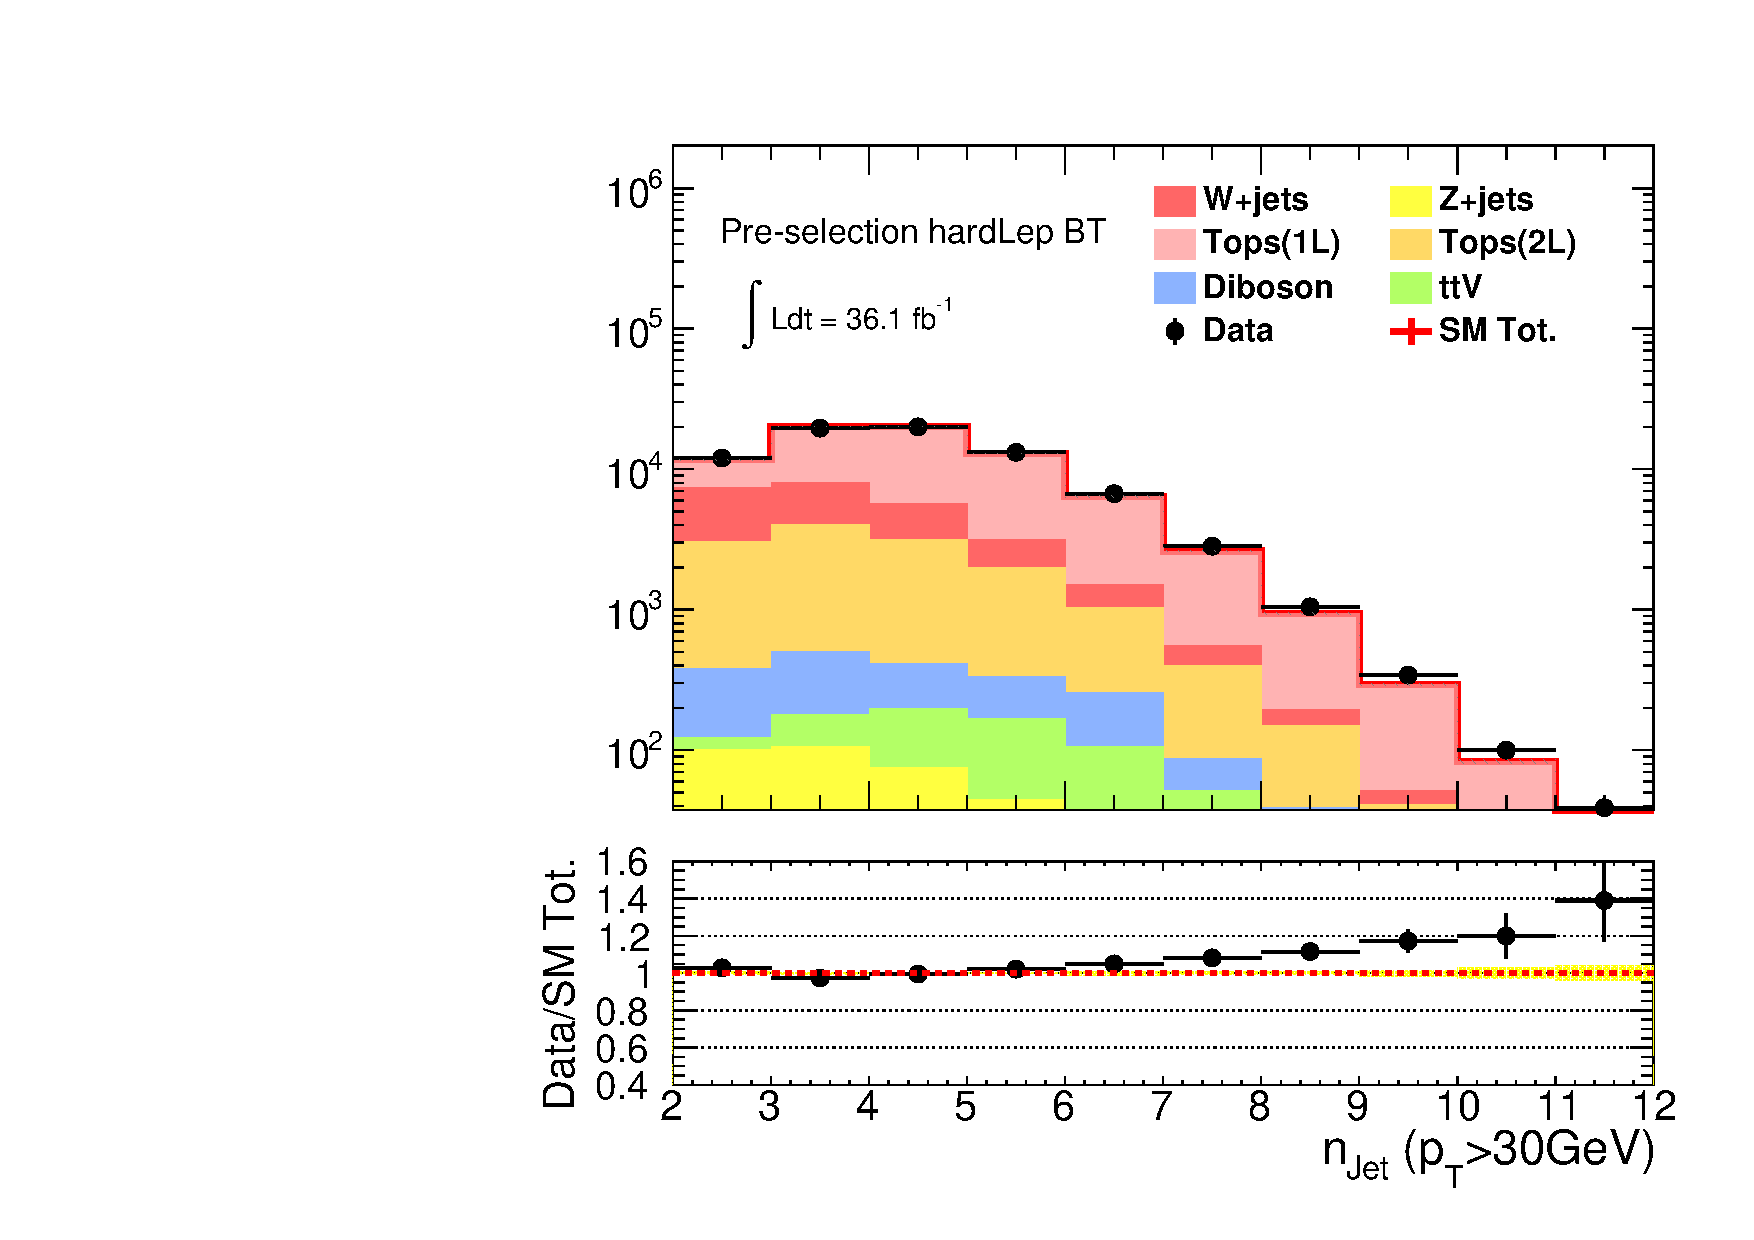
\includegraphics[width=0.48\textwidth]{figures/BGestimation/DataMCComparison/Preselection_hardLepBT/nJet30__Preselection_hardLepBT__rwgt_nJ007_ttPt007.pdf}}
    \subfigure[]{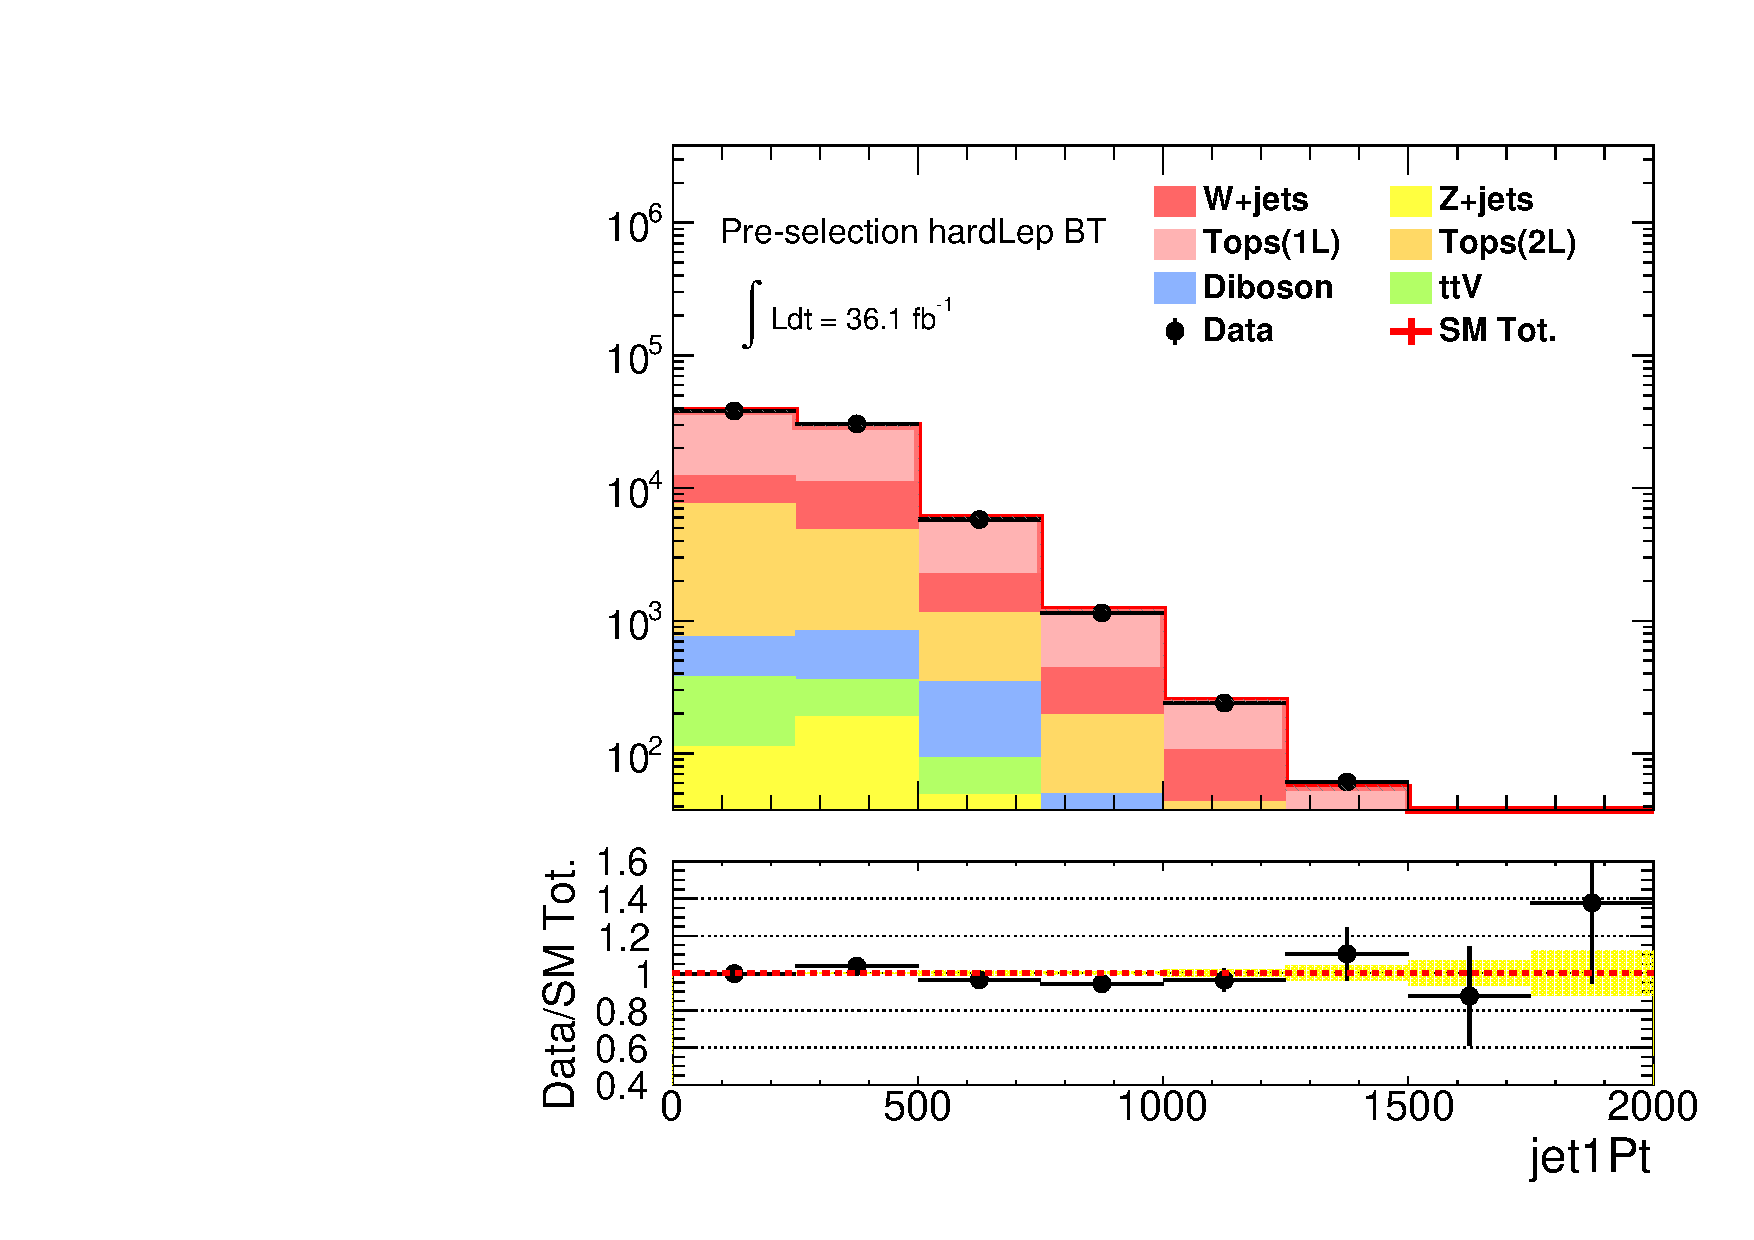
\includegraphics[width=0.48\textwidth]{figures/BGestimation/DataMCComparison/Preselection_hardLepBT/jet1Pt__Preselection_hardLepBT__rwgt_nJ007_ttPt007.pdf}}
    \subfigure[]{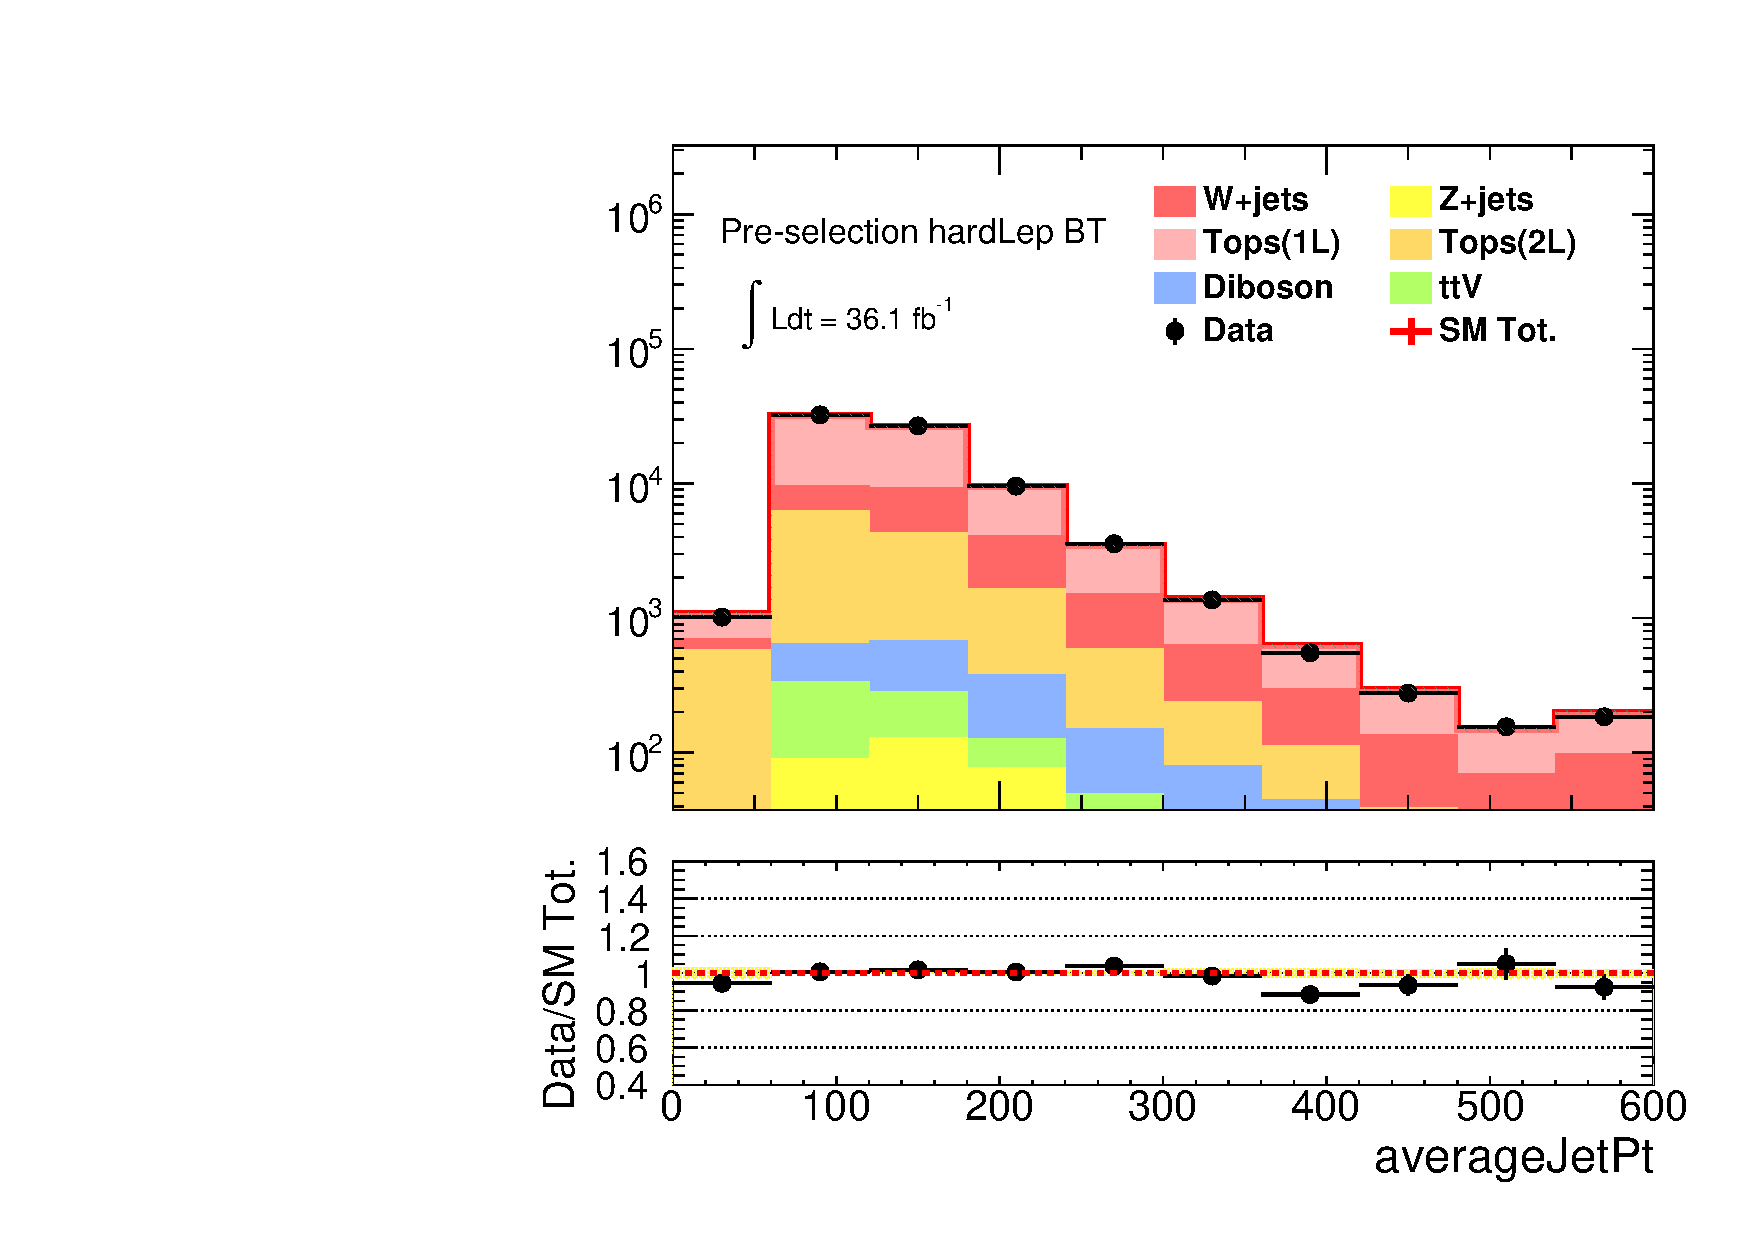
\includegraphics[width=0.48\textwidth]{figures/BGestimation/DataMCComparison/Preselection_hardLepBT/averageJetPt__Preselection_hardLepBT__rwgt_nJ007_ttPt007.pdf}}
    \subfigure[]{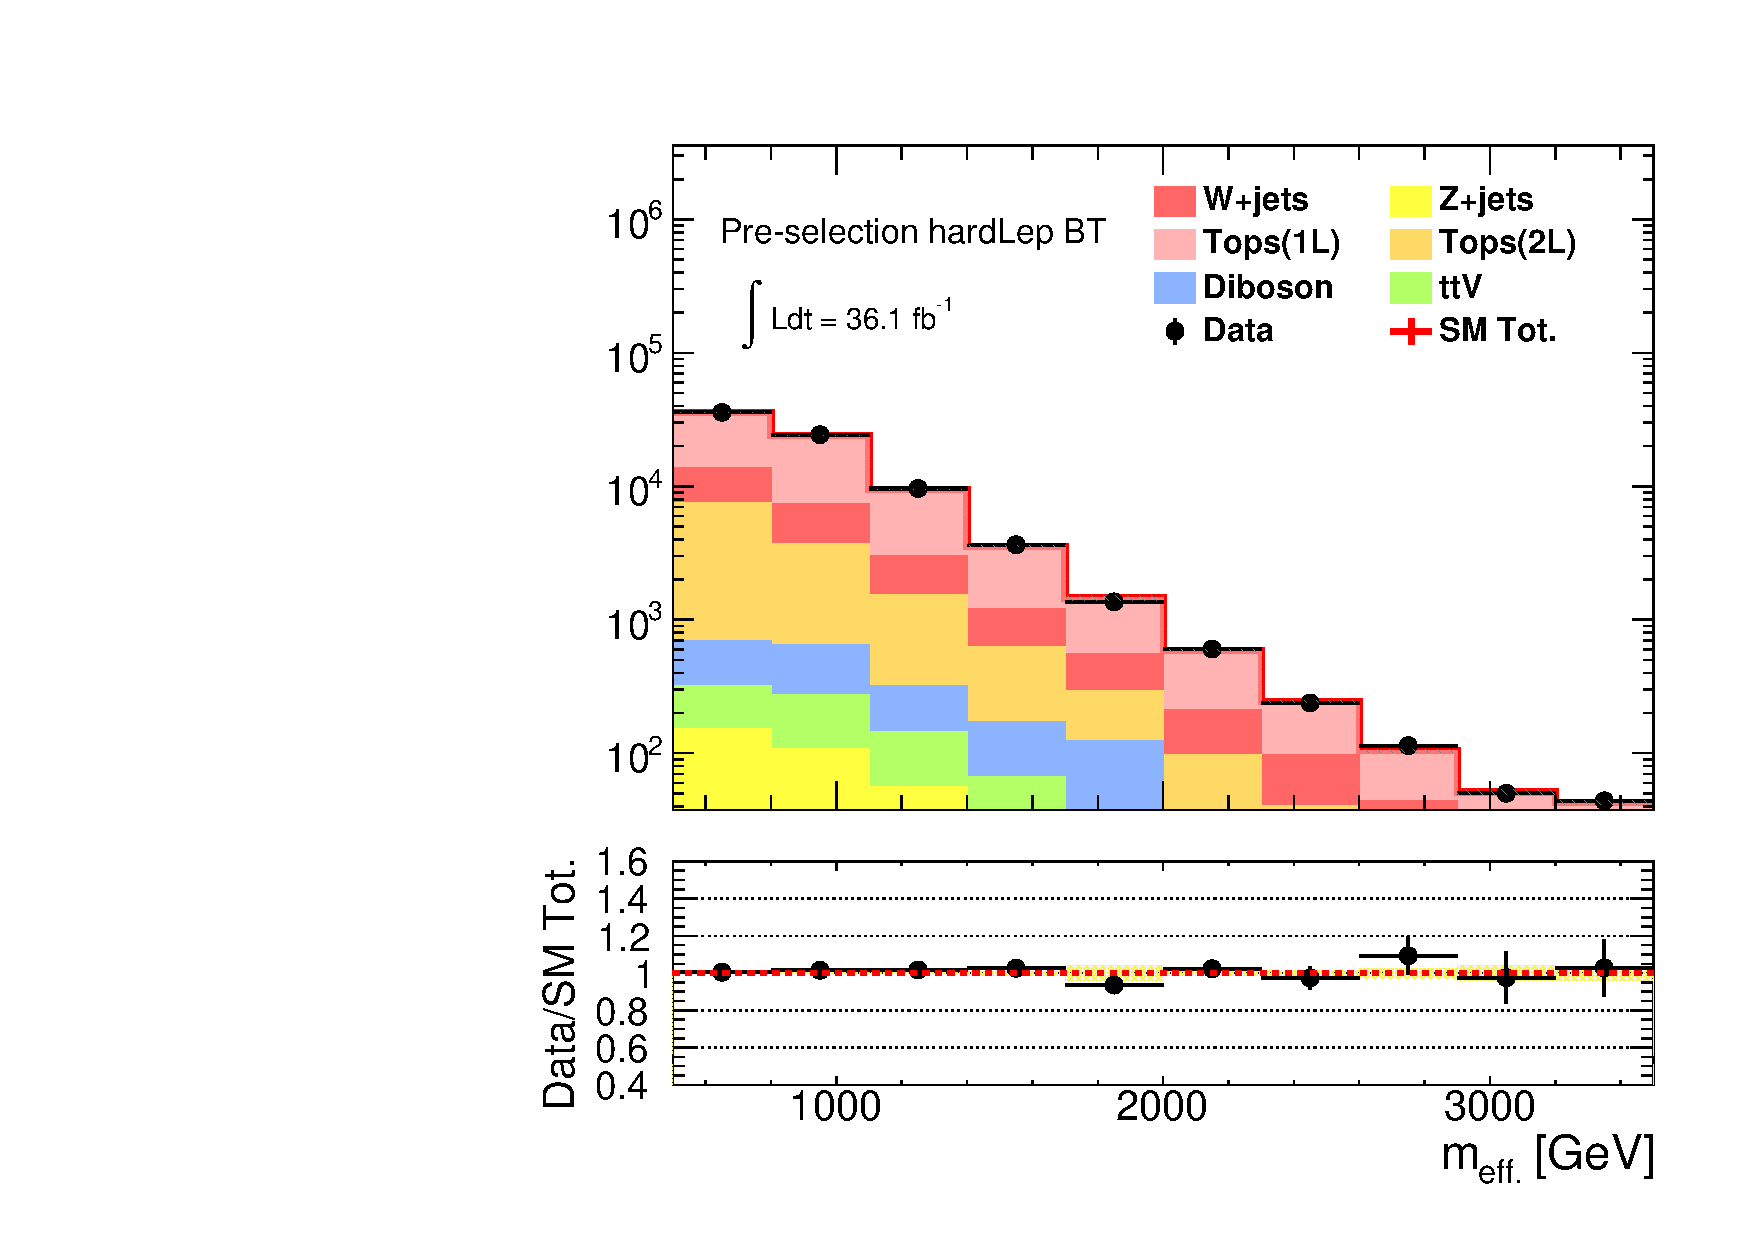
\includegraphics[width=0.48\textwidth]{figures/BGestimation/DataMCComparison/Preselection_hardLepBT/meffInc30__Preselection_hardLepBT__rwgt_nJ007_ttPt007.pdf}}
    \caption{ Kinematical distribution of (a) Jet multiplicity ($p_T>30\gev$) (b) leading-jet pt  (c) average jet pt ($p_T>30\gev$)  (d) $\meffInc$ in the hard lepton b-tagged pre-selection region, with the reweighting $w = 1.05 \times \left[ 1 - 0.061 \,\times p_T(\ttbar) \right]$ (Eq.(\ref{eq::BGestimation::rwgt_ttPt})) being applied for $\ttbar$ MC.
      \label{fig::BGestimation::DataMCPreselHardBT_rwgt1} }
\end{figure}

\begin{figure}[h]
  \centering
    \subfigure[]{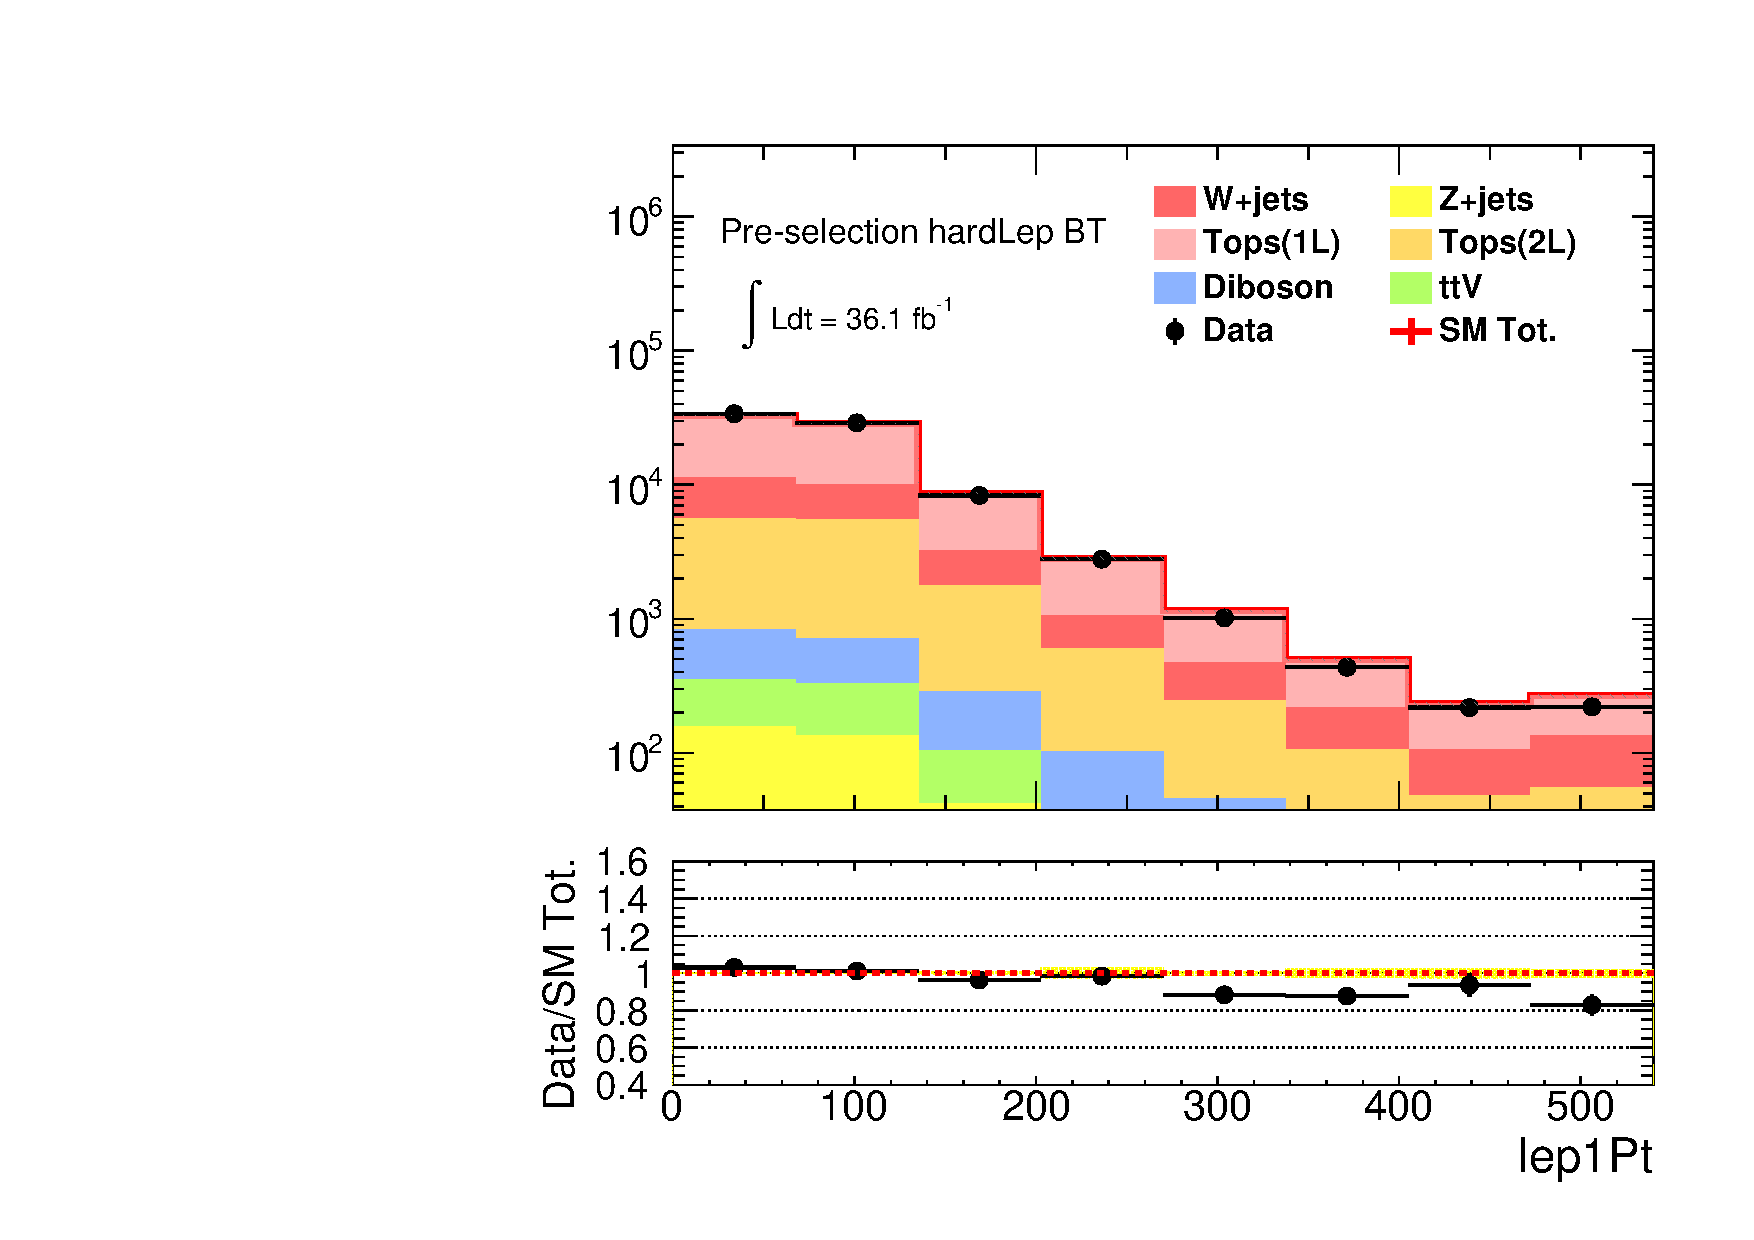
\includegraphics[width=0.48\textwidth]{figures/BGestimation/DataMCComparison/Preselection_hardLepBT/lep1Pt__Preselection_hardLepBT__rwgt_nJ007_ttPt007.pdf}}
    \subfigure[]{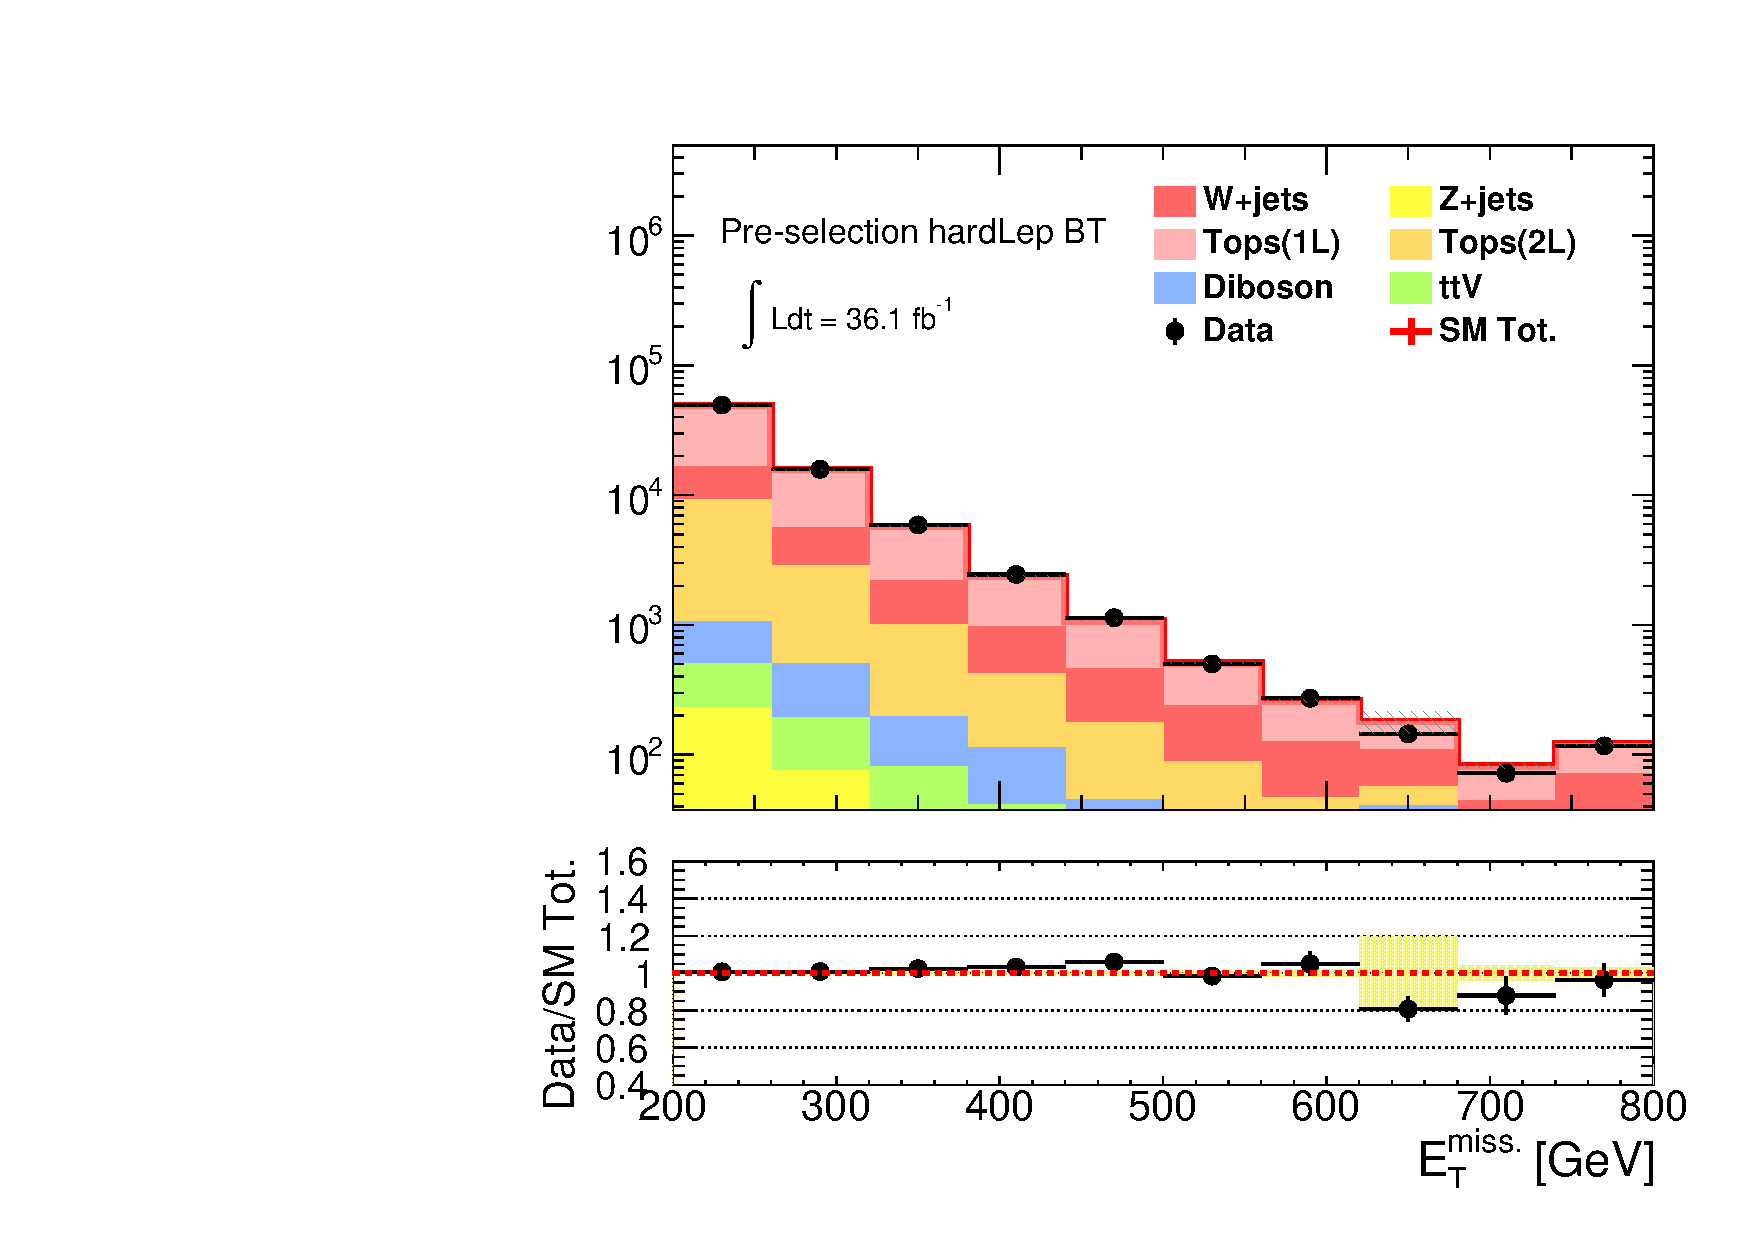
\includegraphics[width=0.48\textwidth]{figures/BGestimation/DataMCComparison/Preselection_hardLepBT/met__Preselection_hardLepBT__rwgt_nJ007_ttPt007.pdf}}
    \subfigure[]{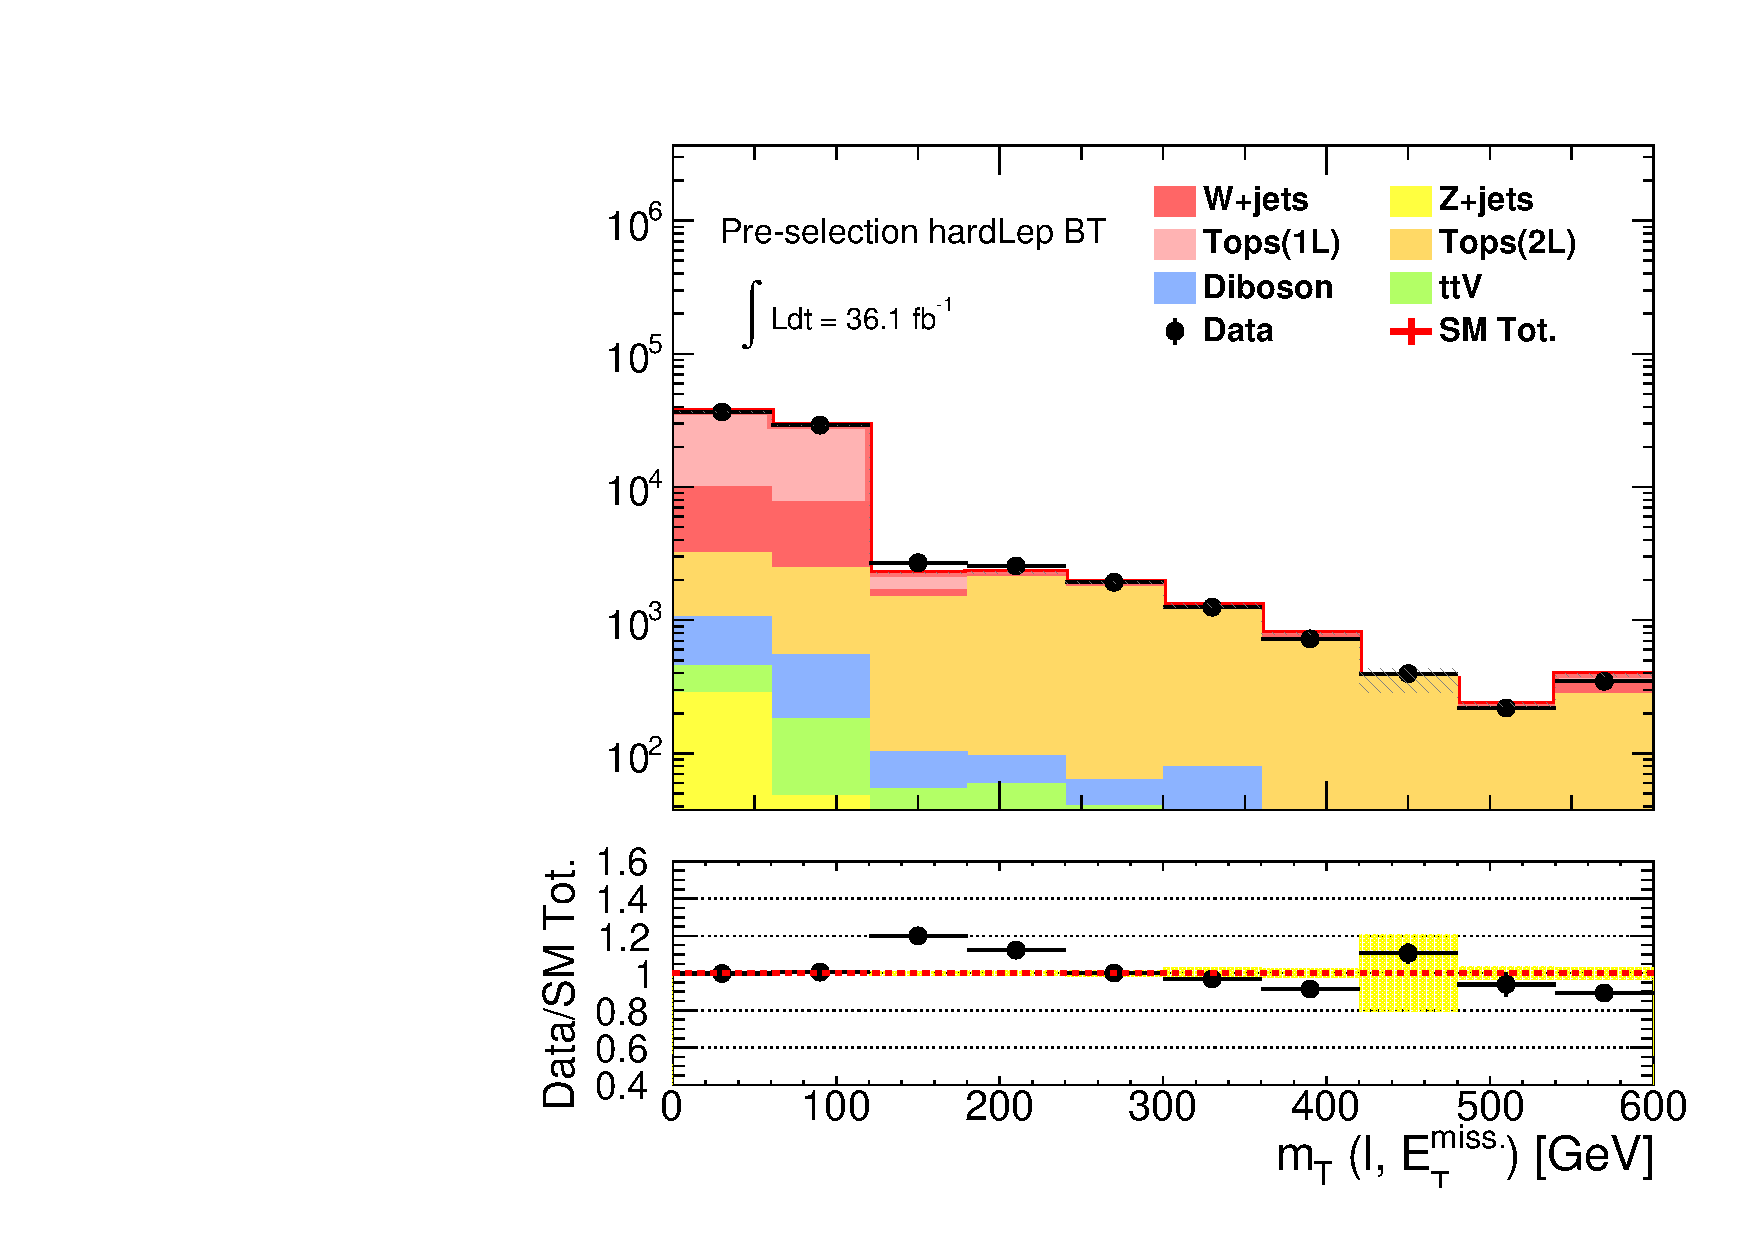
\includegraphics[width=0.48\textwidth]{figures/BGestimation/DataMCComparison/Preselection_hardLepBT/mt__Preselection_hardLepBT__rwgt_nJ007_ttPt007.pdf}}
    \subfigure[]{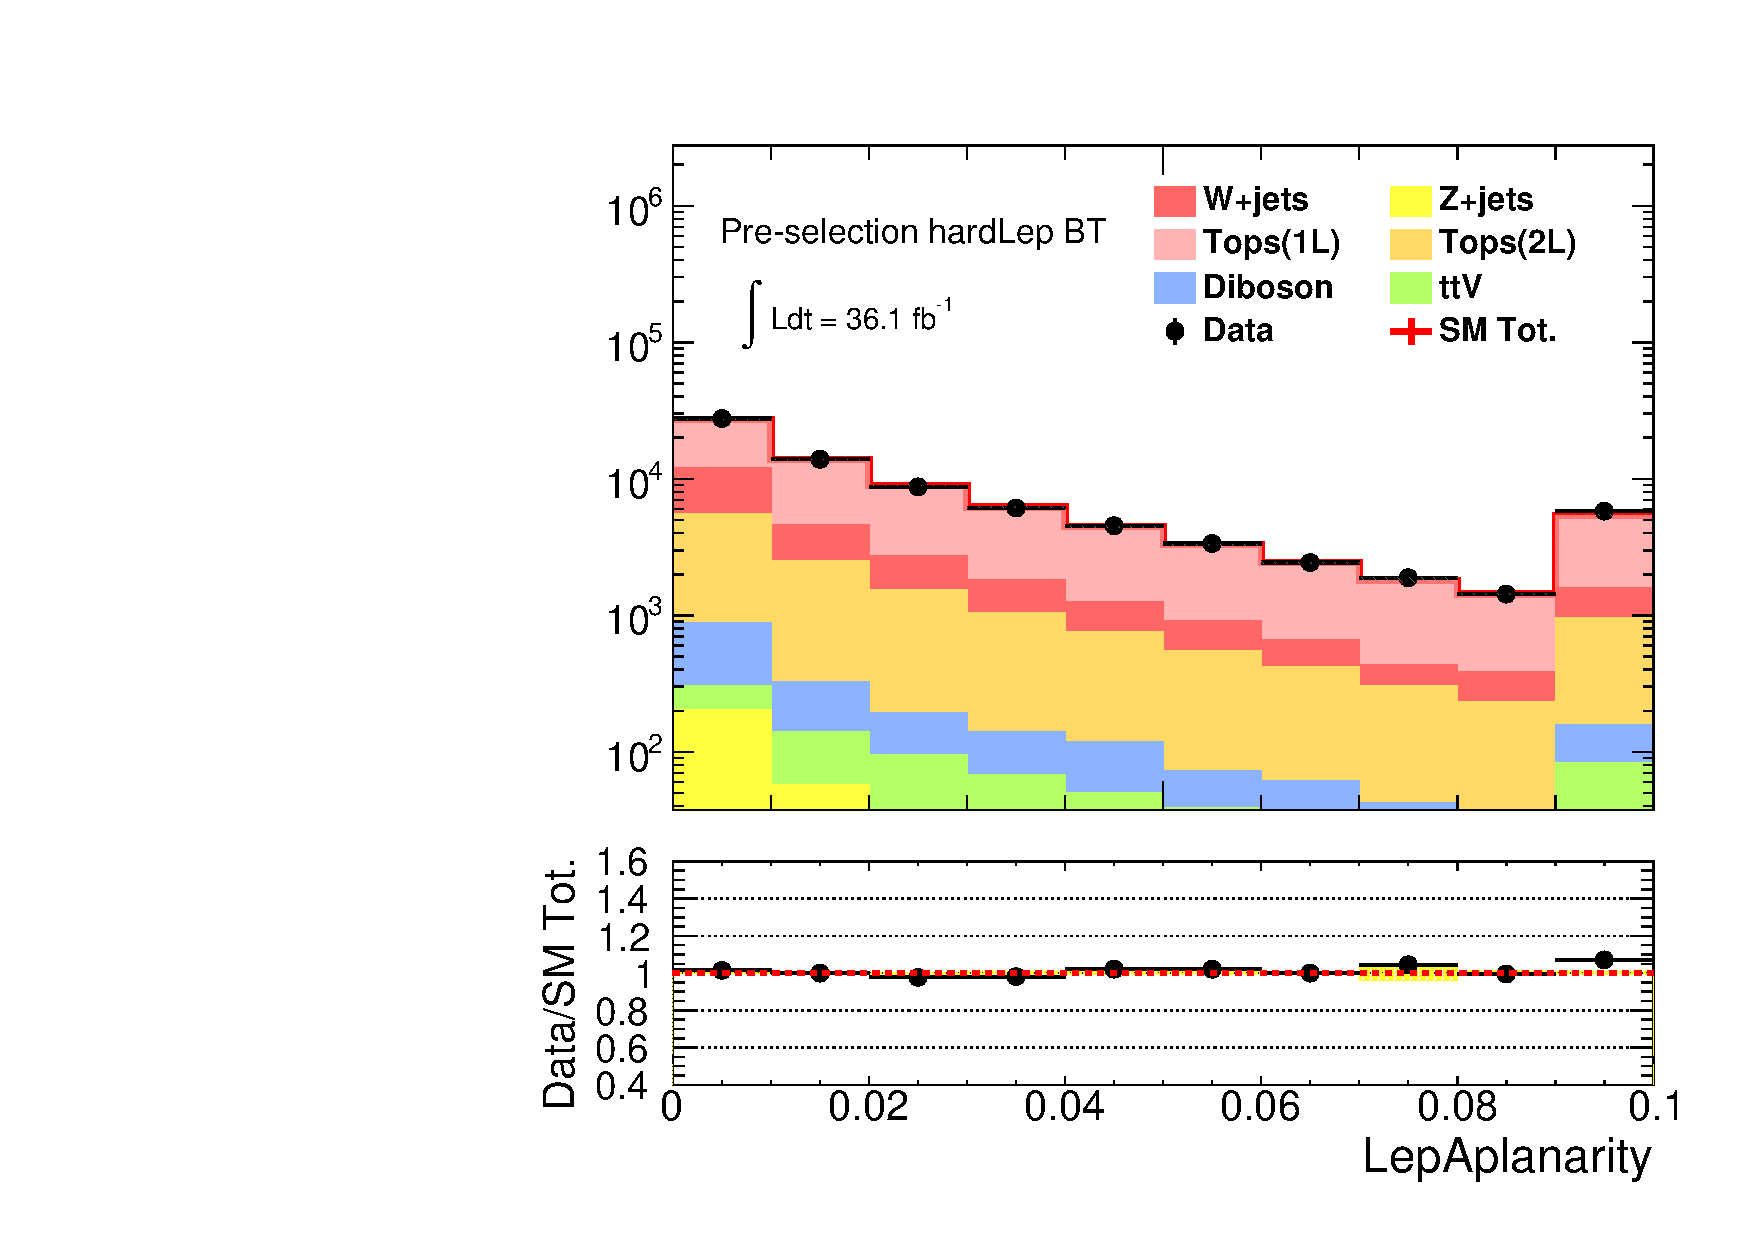
\includegraphics[width=0.48\textwidth]{figures/BGestimation/DataMCComparison/Preselection_hardLepBT/LepAplanarity__Preselection_hardLepBT__rwgt_nJ007_ttPt007.pdf}}
    \caption{ Kinematical distribution of (a) leading-lepton pt (b) $\met$  (c) $\mt$  (d) $\apl$ in the \textbf{hard lepton b-vetoed} pre-selection region, with the reweighting $w = 1.05 \times \left[ 1 - 0.061 \,\times p_T(\ttbar) \right]$ (Eq.(\ref{eq::BGestimation::rwgt_ttPt})) being applied for $\ttbar$ MC.  \label{fig::BGestimation::DataMCPreselHardBT_rwgt2} }
\end{figure}

